% !TeX root = ../../main.tex
\subsection{Control denominators recover interactions under composition shifts}
\label{sec:simcrispr}

We used simCRISPR to generate a factorial knockout-by-treatment screen with a
known guide-level interaction \citep{zhu2026simcrispr}.  Each of three seeds
contained 2,000 sgRNAs and three independent replicates per factorial arm.
Non-targeting guides had a true interaction of zero, and safe-harbor guides
separated the effect of cutting from a targeted gene effect.  Each control
class was split so that normalization and calibration guides were never used
for evaluation.  The benchmark compares denominator choice and moderation
within BARCS. MAGeCK-MLE is a reference with one guide per gene, an input that
lacks within-gene replication for its native gene model and cannot support a
method ranking.

\begin{table}[ht]
\centering
\caption{Interaction recovery in simCRISPR (three-seed mean with standard
deviation in parentheses).  Recall and F1
use targeting guides with $|\mathrm{interaction}|\geq0.2$ as positives.  Null
and safe-harbor rates are held-out call fractions at FDR 0.10.}
\label{tab:simcrispr}
\scriptsize
\setlength{\tabcolsep}{2.5pt}
\begin{tabular}{llrrrr}
\toprule
Method & Denominator & Dir.\ recall & F1 & Null rate & Safe-harbor\\
\midrule
BARCS-ST & Library &
0.376 (0.308) & 0.488 (0.389) & 0.004 (0.008) & 0.002 (0.003)\\
BARCS-MOD & Library &
0.375 (0.323) & 0.481 (0.409) & 0.000 (0.000) & 0.000 (0.000)\\
\midrule
BARCS-ST & Non-targeting &
0.769 (0.094) & 0.870 (0.065) & 0.024 (0.020) & 0.070 (0.025)\\
BARCS-MOD & Non-targeting &
0.838 (0.025) & 0.917 (0.017) & 0.040 (0.040) & 0.080 (0.038)\\
\midrule
BARCS-ST & Safe-harbor &
0.762 (0.087) & 0.864 (0.061) & 0.042 (0.027) & 0.042 (0.008)\\
BARCS-MOD & Safe-harbor &
0.830 (0.019) & 0.914 (0.017) & 0.027 (0.023) &
0.035 (0.005)\\
\midrule
MAGeCK-MLE & Non-targeting &
0.003 (0.001) & 0.006 (0.002) & 0.000 (0.000) & 0.000 (0.000)\\
\bottomrule
\end{tabular}
\end{table}

The full-library denominator preserved effect ranking but shifted the
true-zero guides because widespread depletion increased every surviving
guide's library share.  Their median fitted interaction was 0.184
(interquartile range 0.136--0.231), whereas the corresponding medians were
0.004 and 0.030 for the non-targeting and safe-harbor denominators.  The
control-scale factors were 1.99 and 2.24 for unmoderated and moderated
full-library fits, compared with 1.00--1.07 for the control-denominator fits.
One library-denominator seed collapsed, so the three-seed means in
Table~\ref{tab:simcrispr} poorly describe a typical run.  BARCS-ST F1 was
0.039, 0.709, and 0.716 across the three seeds; BARCS-MOD F1 was 0.011, 0.680,
and 0.754.  With the non-targeting denominator, the corresponding values were
0.798, 0.924, and 0.889 for BARCS-ST and 0.899, 0.933, and 0.920 for
BARCS-MOD. The control denominator improved every seed, with gains that varied
across runs.  In the two noncollapsed runs, F1 was approximately 0.71 versus
0.91, a smaller gain than a near doubling.  The held-out null rates remained
below the nominal 0.10 in all cases.

\begin{figure}[!htbp]
\centering
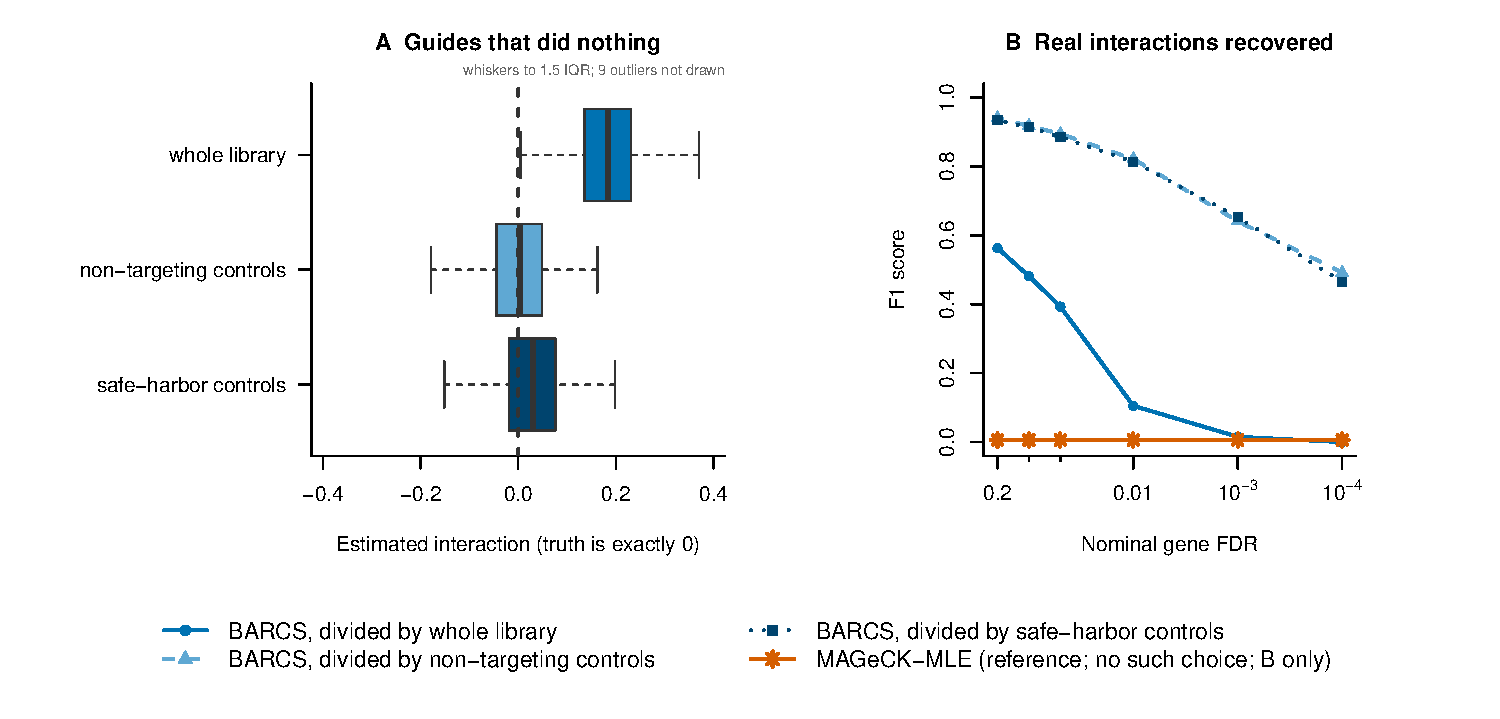
\includegraphics[width=\textwidth]{figures/simcrispr_interaction.pdf}
\caption{\textbf{Denominator choice controls interaction recovery.}  (A)
Estimated interactions among true-zero guides.  A full-library denominator
induces a positive shift; either control denominator removes it.  Boxes span
the interquartile range, whiskers extend to 1.5 times it, and the panel reports the number of observations beyond the whiskers without
plotting those points.
(B) F1 across nominal FDR thresholds; every evaluated threshold is marked.  Control denominators retain
substantially more interaction power.  The three denominator settings share a hue and differ in lightness, line type,
and point shape.  MAGeCK-MLE uses its colour from the other figures and
appears only in (B).}
\label{fig:simcrispr}
\end{figure}

Figure~\ref{fig:simcrispr} shows the composition-induced null shift and
threshold curves.  Although the control denominators performed similarly
overall, they differed in their handling of cutting artifacts.  Safe-harbor
guides were called at 0.080 after non-targeting normalization and 0.035 after
safe-harbor normalization. In these simulations, both control classes
supported targeted-interaction recovery, while safe-harbor normalization
absorbed more of the shared cutting response.  A comparison of gene-level
interaction methods would require several independently simulated guides per
gene and a common gene-level interaction estimand.
